\documentclass{beamer}
\usetheme{metropolis}

\usepackage[spanish]{babel}
\usepackage[utf8]{inputenc}
\usepackage{tikz}
\usepackage{xcolor}
\usepackage{amsmath}
\usepackage{listings}

% Definición de colores personalizados
\definecolor{primary}{RGB}{46, 204, 113}
\definecolor{secondary}{RGB}{52, 152, 219}
\definecolor{accent}{RGB}{231, 76, 60}
\definecolor{background}{RGB}{236, 240, 241}
\definecolor{gradient1}{RGB}{255, 107, 107}
\definecolor{gradient2}{RGB}{255, 159, 67}

% Configuración del tema
\setbeamercolor{normal text}{fg=black,bg=background}
\setbeamercolor{structure}{fg=primary}
\setbeamercolor{alerted text}{fg=accent}

\definecolor{lightgray}{rgb}{0.95,0.95,0.95}
\definecolor{darkgreen}{rgb}{0,0.5,0}
\definecolor{darkblue}{rgb}{0,0,0.5}

\lstset{
  backgroundcolor=\color{lightgray},
  basicstyle=\tiny\ttfamily,
  keywordstyle=\color{darkblue}\bfseries,
  commentstyle=\color{darkgreen},
  stringstyle=\color{red},
  numbers=left,
  numberstyle=\tiny\color{gray},
  stepnumber=1,
  numbersep=5pt,
  showspaces=false,
  showstringspaces=false,
  showtabs=false,
  frame=single,
  tabsize=2,
  language=Python,
  breaklines=true,
  breakatwhitespace=true
}


\title{\Huge\textbf{Probabilidad y Estadística para I.O.}}
\subtitle{Investigación Operativa}
\author{Universidad de San Andrés}
\date{}


\begin{document}

\begin{frame}
    \titlepage
\end{frame}

\begin{frame}{Fundamentos de Probabilidad}
    \begin{itemize}
        \item La probabilidad es fundamental en IO para:
        \begin{itemize}
            \item Optimizar inventarios con demanda aleatoria
            \item Evaluar riesgos en proyectos
            \item Modelar tiempos de espera en colas
            \item Analizar confiabilidad de sistemas
        \end{itemize}
    \end{itemize}
\end{frame}

\begin{frame}{Conceptos Básicos}
    \begin{itemize}
        \item \textbf{Experimento aleatorio:} Proceso con resultado impredecible
        \item \textbf{Espacio muestral ($\Omega$):} Conjunto de resultados posibles
        \item \textbf{Evento:} Subconjunto del espacio muestral
    \end{itemize}
\end{frame}

\begin{frame}{Propiedades y Teoremas}
    Para eventos $A$ y $B$ en $\Omega$:
    \begin{itemize}
        \item $0 \leq P(A) \leq 1$, $P(\Omega) = 1$, $P(\emptyset) = 0$
        \item $P(A \cup B) = P(A) + P(B) - P(A \cap B)$
        \item Probabilidad condicional: $P(A|B) = \frac{P(A \cap B)}{P(B)}$
        \item Independencia: $P(A \cap B) = P(A)P(B)$
        \item Teorema de Bayes: $P(A|B) = \frac{P(B|A)P(A)}{P(B)}$
    \end{itemize}
\end{frame}

\begin{frame}{Variables Aleatorias}
    \begin{itemize}
        \item \textbf{Discretas:} Valores específicos y aislados
        \begin{itemize}
            \item Llegadas a un banco por hora
            \item Productos defectuosos en un lote
            \item Intentos hasta primer éxito
        \end{itemize}
        \item \textbf{Continuas:} Valores en rango continuo
        \begin{itemize}
            \item Tiempo de servicio
            \item Peso de un producto
            \item Distancia recorrida
        \end{itemize}
    \end{itemize}
\end{frame}

\begin{frame}{Control de Calidad - Binomial}
    \textbf{Problema:}
    
    Una empresa fabrica lotes de 1200 tornillos. Se sabe que el 3\% de los tornillos son defectuosos. Para controlar la calidad, se toma una muestra aleatoria de 50 tornillos. El lote se rechaza si se encuentran más de 2 tornillos defectuosos en la muestra. \textbf{¿Cuál es la probabilidad de que un lote con 3\% de defectuosos sea rechazado?}
    
    \textbf{Modelo:}
    \begin{itemize}
        \item $X \sim \text{Binomial}(50, 0.03)$
        \item $P(X > 2) = 1 - P(X \leq 2)$
    \end{itemize}
\end{frame}

\begin{frame}{Control de Calidad - Solución}
    \[P(X = k) = \binom{n}{k} p^k (1-p)^{n-k}\]
    
    Para $n = 50$, $p = 0.03$:
    \begin{align*}
        P(X=0) &\approx 0.218 \\
        P(X=1) &\approx 0.337 \\
        P(X=2) &\approx 0.266 \\
        P(X \leq 2) &\approx 0.821 \\
        P(X > 2) &= 0.179
    \end{align*}
\end{frame}

\begin{frame}[fragile]{Control de Calidad - Python}
    \begin{lstlisting}
from scipy.stats import binom

# Parametros
n = 50      # Tamano de la muestra
p = 0.03    # Probabilidad de defecto

# Probabilidad de rechazar el lote
prob_rechazo = 1 - binom.cdf(2, n, p)
print(f"Probabilidad de rechazar el lote: {prob_rechazo:.4f}")
    \end{lstlisting}
\end{frame}

\begin{frame}{Colas - Poisson}
    \textbf{Problema:}
    
    En un centro de distribución, los pedidos llegan con una tasa media de 8 pedidos por hora. El sistema colapsa si se reciben más de 10 pedidos en una hora. \textbf{¿Cuál es la probabilidad de que el sistema colapse?}
    
    \textbf{Modelo:}
    \begin{itemize}
        \item $X \sim \text{Poisson}(8)$
        \item Calcular $P(X > 10)$
    \end{itemize}
\end{frame}

\begin{frame}{Colas - Solución}
    Para $\lambda = 8$:
    \begin{align*}
        P(X \leq 10) &= \sum_{k=0}^{10} \frac{8^k e^{-8}}{k!} \approx 0.815 \\
        P(X > 10) &= 1 - 0.815 = 0.185
    \end{align*}
\end{frame}

\begin{frame}[fragile]{Colas - Python}
    \begin{lstlisting}
from scipy.stats import poisson

# Parametros
lambd = 8   # Tasa de pedidos por hora

# Probabilidad de colapso
prob_colapso = 1 - poisson.cdf(10, lambd)
print(f"Probabilidad de colapso: {prob_colapso:.4f}")
    \end{lstlisting}
\end{frame}

\begin{frame}{Contratos - Normal}
    \textbf{Problema:}
    
    El tiempo de fabricación tiene una media de 120 minutos y desviación estándar de 15 minutos. Un contrato exige que la pieza se produzca en menos de 100 minutos. \textbf{¿Con qué porcentaje de las veces se incumplirá el contrato?}
    
    \textbf{Modelo:}
    \begin{itemize}
        \item $X \sim N(120, 15^2)$
        \item Calcular $P(X > 100)$
    \end{itemize}
\end{frame}

\begin{frame}{Contratos - Solución}
    \begin{align*}
        P(X > 100) &= 1 - P(X < 100) \\
        &= 1 - P\left(Z < \frac{100-120}{15}\right) \\
        &\Rightarrow 1 - P(Z < -1.33) \\
        &= P(Z > -1.33) \\
        &\approx 0.9082
    \end{align*}
\end{frame}

\begin{frame}[fragile]{Contratos - Python}
    \begin{lstlisting}
from scipy.stats import norm

# Parametros
mu = 120      # Media del tiempo de fabricacion
sigma = 15    # Desviacion estandar

# Probabilidad de incumplir contrato: P(X > 100)
prob_incumplimiento = 1 - norm.cdf(100, loc=mu, scale=sigma)
print(f"Probabilidad de incumplimiento del contrato: {prob_incumplimiento:.4f}")
    \end{lstlisting}
\end{frame}

\begin{frame}{Monte Carlo}
    \textbf{Pasos:}
    \begin{enumerate}
        \item Identificar variables aleatorias
        \item Elegir distribuciones
        \item Generar muestras
        \item Ejecutar modelo
        \item Analizar resultados
    \end{enumerate}
\end{frame}

\begin{frame}{Inventario - Problema}
    \textbf{Problema:}
    
    Una tienda vende un producto cuya demanda diaria sigue una distribución normal con media 80 unidades y desviación estándar 10 unidades. Cada semana decide cuántas unidades pedir.
    
    \textbf{Costos:}
    \begin{itemize}
        \item Mantener stock: \$2/unidad
        \item Faltante: \$5/unidad
        \item Venta: \$20/unidad
        \item Compra: \$10/unidad
    \end{itemize}
    
    \textbf{Objetivo:} Encontrar el nivel de pedido semanal óptimo que maximiza el beneficio esperado.
\end{frame}

\begin{frame}[fragile]{Inventario - Python (Parte 1)}
    \begin{lstlisting}[language=Python]
import numpy as np
import matplotlib.pyplot as plt

# Parametros del problema
media_demanda = 80
desvio_demanda = 10
precio_venta = 20
costo_unitario = 10
costo_inventario = 2
costo_faltante = 5
semanas = 1000
np.random.seed(42)  # Para reproducibilidad
niveles_pedido = np.arange(60, 121, 1)  # De 60 a 120 unidades
beneficio_promedio = []
    \end{lstlisting}
\end{frame}

\begin{frame}[fragile]{Inventario - Python (Parte 2)}
    \begin{lstlisting}[language=Python]
# Simulacion Monte Carlo
for Q in niveles_pedido:
    demanda_simulada = np.random.normal(media_demanda, desvio_demanda, semanas).round().astype(int)
    demanda_simulada = np.maximum(demanda_simulada, 0)  # No hay demanda negativa
    ventas = np.minimum(Q, demanda_simulada)
    stock_sobrante = np.maximum(Q - demanda_simulada, 0)
    faltantes = np.maximum(demanda_simulada - Q, 0)
    beneficio = (ventas * precio_venta) - (Q * costo_unitario) - \
                (stock_sobrante * costo_inventario) - (faltantes * costo_faltante)
    beneficio_promedio.append(np.mean(beneficio))

plt.plot(niveles_pedido, beneficio_promedio)
plt.xlabel('Nivel de pedido semanal (Q)')
plt.ylabel('Beneficio promedio ($)')
plt.title('Simulacion Monte Carlo - Beneficio vs Nivel de Pedido')
plt.axvline(niveles_pedido[np.argmax(beneficio_promedio)], color='r', 
           linestyle='--', label=f'Optimo: {niveles_pedido[np.argmax(beneficio_promedio)]} unidades')
plt.legend()
plt.show()
    \end{lstlisting}
\end{frame}

\begin{frame}{Resultado de la Simulación}
    \begin{center}
        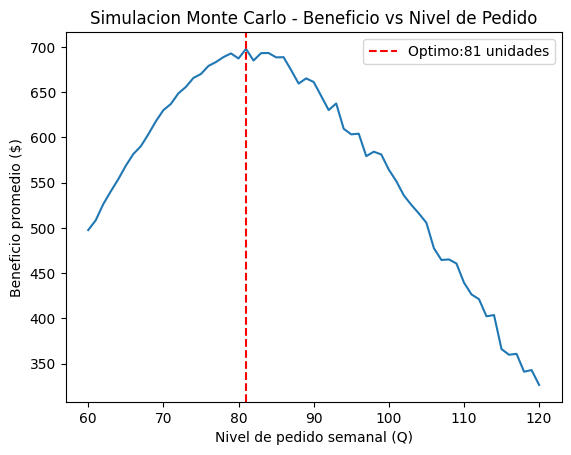
\includegraphics[width=0.7\textwidth]{montecarlo.png}
    \end{center}
\end{frame}

\begin{frame}{Repaso Probabilidad}
    \begin{center}
        \Large{¿Preguntas?}
    \end{center}
\end{frame}

\end{document} 